\documentclass[a4paper]{scrartcl}

% UTF-8 encoding
\usepackage[utf8]{inputenc}

% include 
\usepackage{graphicx}

% Meta informations
\title{4 Stereo Matching}
\subtitle{Computer Vision practical seminar \\ TU Dresden}
\author{Lucas Kahlert}
\date{\today}

\begin{document}

\maketitle

\section{Stereo block matching}

For the different matching criteria and block size post processing was
enabled. That includes left-right-consistency (LRC) with an threshold of 3px
for the difference between the left and right flow and median filtering with a
filter radius of 1px.

% input images


\subsection{Matching criteria}

The results of the different matching criteria are very similar. Therefore we
use SSD (figure \ref{fig:disparity-r2-ssd-d20-m1}) because it has a little bit fewer artifacts than SAD (figure \ref{fig:disparity-r2-sad-d20-m1}) and is faster
then cross correlation. (figure \ref{fig:disparity-r2-ccr-d20-m1})

\vspace{1cm}
\begin{minipage}{0.8\textwidth}
  \centering
  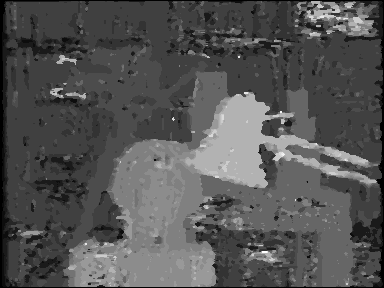
\includegraphics[width=0.8\textwidth]{disparity-r1-ssd-d20-m1.png}
  \captionof{figure}{SSD}
  \label{fig:disparity-r2-ssd-d20-m1}
\end{minipage}

\vspace{1cm}
\begin{minipage}{0.8\textwidth}
  \centering
  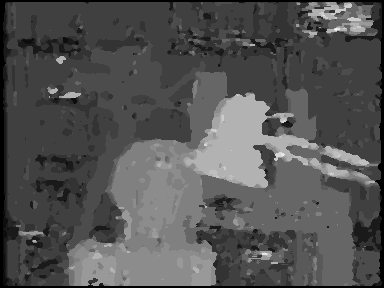
\includegraphics[width=0.8\textwidth]{disparity-r2-sad-d20-m1.png}
  \captionof{figure}{SAD}
  \label{fig:disparity-r2-sad-d20-m1}
\end{minipage}

\vspace{1cm}
\begin{minipage}{0.8\textwidth}
  \centering
  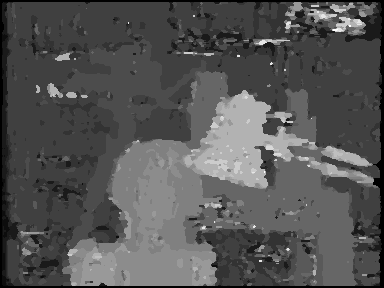
\includegraphics[width=0.8\textwidth]{disparity-r2-ccr-d20-m1.png}
  \captionof{figure}{Cross Correlation}
  \label{fig:disparity-r2-ccr-d20-m1}
\end{minipage}


\subsection{Block Size}

With small block size you can see more details but the disparity map is very
noisy. Large block sizes matches the better but decreases the details. If the
block size is large enough that also untextured areas are matched, the
disparity map has nearly no noise. But the details (for example the camera in
the background) are hardly to recognize.

\vspace{1cm}
\begin{minipage}{0.8\textwidth}
  \centering
  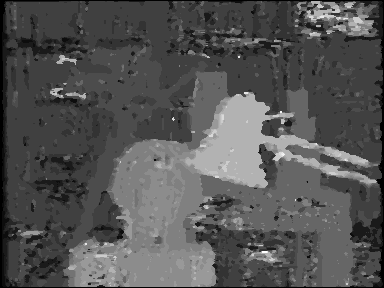
\includegraphics[width=0.8\textwidth]{disparity-r1-ssd-d20-m1.png}
  \captionof{figure}{Block size 3}
  \label{fig:disparity-r1-ssd-d20-m1}
\end{minipage}

\vspace{1cm}
\begin{minipage}{0.8\textwidth}
  \centering
  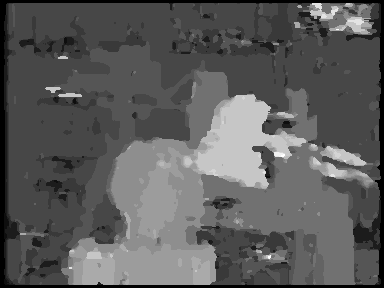
\includegraphics[width=0.8\textwidth]{disparity-r3-ssd-d20-m1.png}
  \captionof{figure}{Block size 7}
  \label{fig:disparity-r3-ssd-d20-m1}
\end{minipage}

\vspace{1cm}
\begin{minipage}{0.8\textwidth}
  \centering
  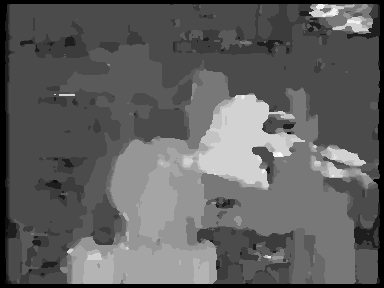
\includegraphics[width=0.8\textwidth]{disparity-r4-ssd-d20-m1.png}
  \captionof{figure}{Block size 9}
  \label{fig:disparity-r4-ssd-d20-m1}
\end{minipage}

\vspace{1cm}
\begin{minipage}{0.8\textwidth}
  \centering
  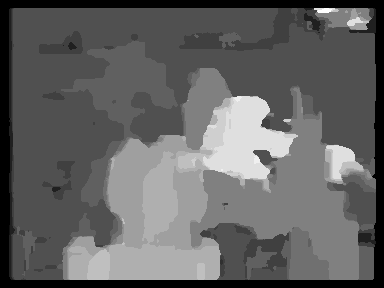
\includegraphics[width=0.8\textwidth]{disparity-r8-ssd-d20-m1.png}
  \captionof{figure}{Block size 17}
  \label{fig:disparity-r8-ssd-d20-m1}
\end{minipage}

\vspace{1cm}
\begin{minipage}{0.8\textwidth}
  \centering
  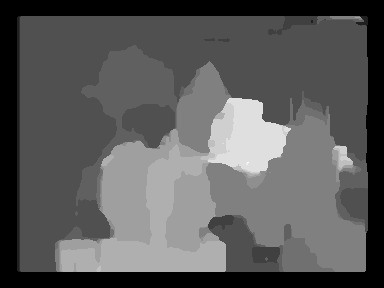
\includegraphics[width=0.8\textwidth]{disparity-r16-ssd-d20-m1.png}
  \captionof{figure}{Block size 33}
  \label{fig:disparity-r16-ssd-d20-m1}
\end{minipage}


\subsection{Maximal disparity}

The maximal disparity should be larger than the real maximal disparity
occuring in the image. A small maximal disparity increases the compution time.

If you increase the maximal disparity the whole disparity map will get a
little bit darker because in some outliers it will reach the maximal disparity
and the normalization will decrease all other points.

\vspace{1cm}
\begin{minipage}{0.8\textwidth}
  \centering
  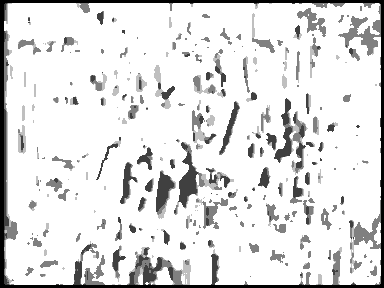
\includegraphics[width=0.8\textwidth]{disparity-r3-ssd-d4-m1.png}
  \captionof{figure}{Maximal disparity of 4px}
  \label{fig:disparity-r3-ssd-d4-m1}
\end{minipage}

\vspace{1cm}
\begin{minipage}{0.8\textwidth}
  \centering
  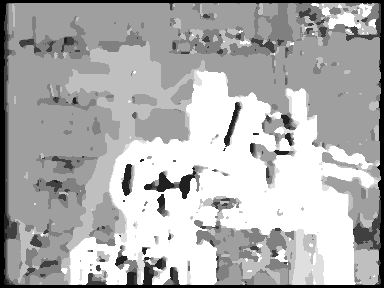
\includegraphics[width=0.8\textwidth]{disparity-r3-ssd-d8-m1.png}
  \captionof{figure}{Maximal disparity of 8px}
  \label{fig:disparity-r3-ssd-d8-m1}
\end{minipage}

\vspace{1cm}
\begin{minipage}{0.8\textwidth}
  \centering
  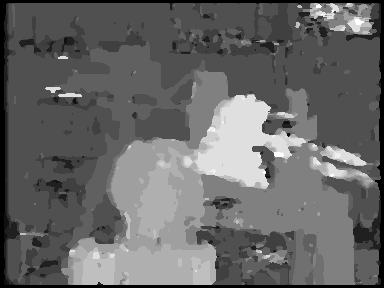
\includegraphics[width=0.8\textwidth]{disparity-r3-ssd-d16-m1.png}
  \captionof{figure}{Maximal disparity of 16px}
  \label{fig:disparity-r3-ssd-d16-m1}
\end{minipage}

\vspace{1cm}
\begin{minipage}{0.8\textwidth}
  \centering
  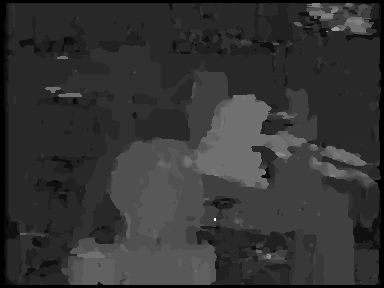
\includegraphics[width=0.8\textwidth]{disparity-r3-ssd-d32-m1.png}
  \captionof{figure}{Maximal disparity of 32px}
  \label{fig:disparity-r3-ssd-d32-m1}
\end{minipage}

\vspace{1cm}
\begin{minipage}{0.8\textwidth}
  \centering
  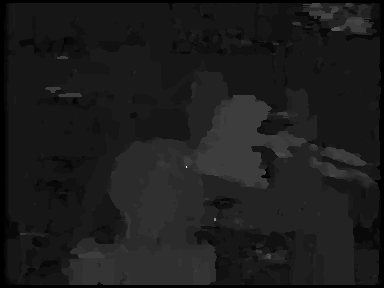
\includegraphics[width=0.8\textwidth]{disparity-r3-ssd-d64-m1.png}
  \captionof{figure}{Maximal disparity of 64px}
  \label{fig:disparity-r3-ssd-d64-m1}
\end{minipage}



\section{Support block size with ground truth}

\vspace{1cm}
\begin{minipage}{0.8\textwidth}
  \centering
    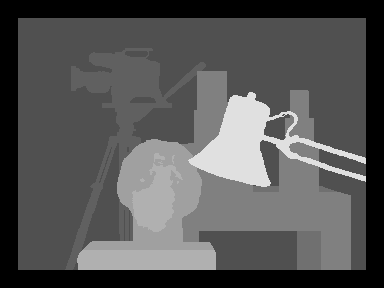
\includegraphics[width=0.8\textwidth]{../lab_4_stereo_matching/GT.png}
    \captionof{figure}{Ground truth}
\end{minipage}

\vspace{1cm}
\begin{minipage}{0.8\textwidth}
  \centering
    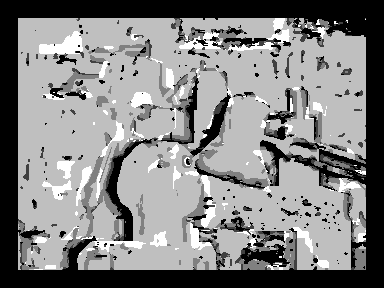
\includegraphics[width=0.8\textwidth]{opt-block-size.png}
    \captionof{figure}{Optimal block sizes}
\end{minipage}

\vspace{1cm}
\begin{minipage}{0.8\textwidth}
  \centering
    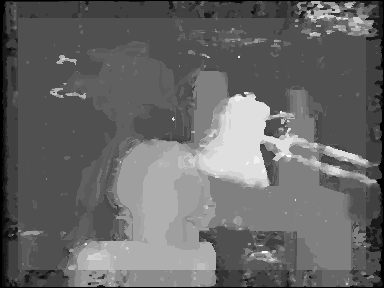
\includegraphics[width=0.8\textwidth]{disparity-gt-ssd-d20-m1.png}
    \captionof{figure}{Matching with optimal block sizes}
\end{minipage}


\section{3D point cloud}

\begin{minipage}{0.8\textwidth}
  \centering
    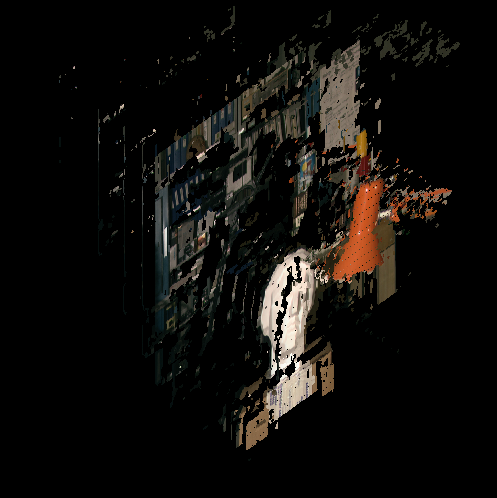
\includegraphics[width=0.7\textwidth]{point-cloud-4.png}
    \captionof{figure}{3D point cloud of disparity map in figure \ref{fig:disparity-r3-ssd-d20-m1}}
\end{minipage}

\vspace{1cm}
\begin{minipage}{0.8\textwidth}
  \centering
    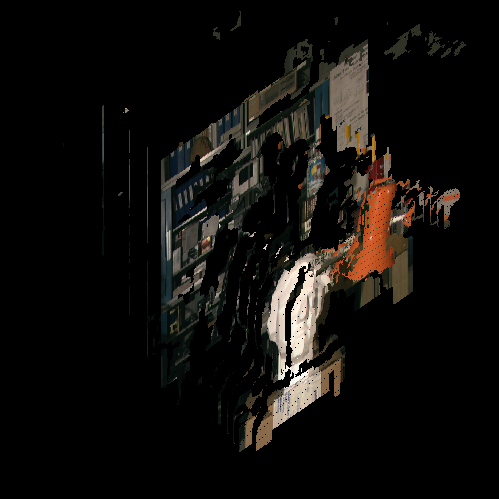
\includegraphics[width=0.7\textwidth]{point-cloud-3.png}
    \captionof{figure}{3D point cloud of disparity map in figure \ref{fig:disparity-r8-ssd-d20-m1}}
\end{minipage}


\section{Optical Flow}

The optical flow is normalized and displayed in the HSV color spaces.

\vspace{1cm}
\begin{minipage}{0.8\textwidth}
  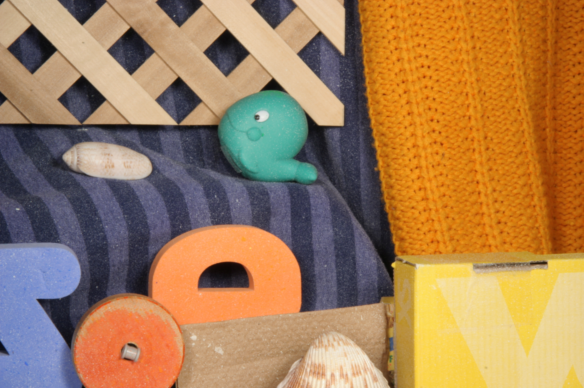
\includegraphics[width=0.5\textwidth]{../lab_4_optical_flow/frame10.png}
  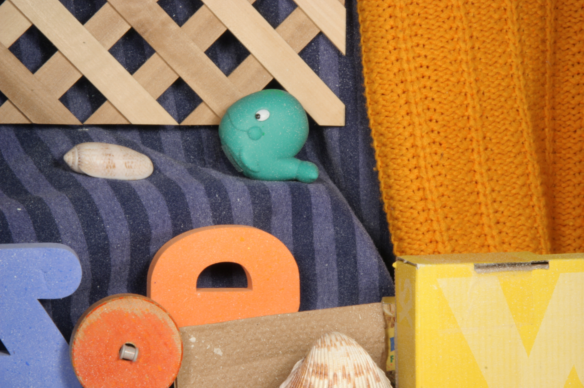
\includegraphics[width=0.5\textwidth]{../lab_4_optical_flow/frame11.png}
  \captionof{figure}{Input frames}
\end{minipage}

\vspace{1cm}
\begin{minipage}{0.8\textwidth}
  \centering
    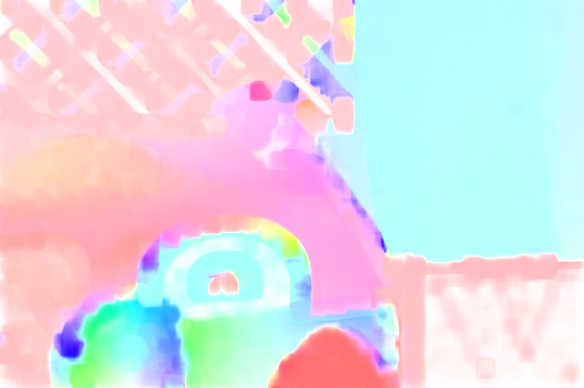
\includegraphics[width=0.8\textwidth]{optical_flow.png}
    \captionof{figure}{Optical flow}
\end{minipage}

\end{document}